\documentclass{article}
\usepackage{fontspec}\defaultfontfeatures{Ligatures=TeX}
\usepackage{setspace}\setstretch{1.3} % \begin{spacing}{1.3}
\usepackage[a4paper,vmargin={1.5cm,2.5cm},hmargin={1.5cm,1.5cm}]{geometry}
%-----------------------------------------------------------------------------%
\usepackage{settings}
%-----------------------------------------------------------------------------%
%%% Title %%%
\title{一個關於剪紙的定理}
\author{Jesse C.\ Chen\thanks{Contact: \texttt{jessekelighine.com}}}
\date{\texttt{\today}}
%-----------------------------------------------------------------------------%

\begin{document}
\begin{multicols*}{2}

\maketitle

\noindent

\begin{definition}[圖形]
	一個圖形是一個簡單多邊形,亦即:
	一個圖形沒有洞,並且其邊不與自己相交。
\end{definition}
\begin{remark}
	簡單來說,就是可以用一張紙剪出來且沒有洞的圖形。
\end{remark}

\begin{definition}[剪]
	\underdot{剪}指將一個圖形以一條\underdot{直線}分割成兩部分。
\end{definition}
\begin{remark}
	這個定義模仿的就是一把剪刀剪下去的概念。
\end{remark}

\begin{definition}[貼]
	\underdot{貼}指的是把兩個圖形\underdot{不重疊地}合併再一起。
\end{definition}

\begin{definition}[剪貼]
	\underdot{剪貼}指的是對一個圖形先進行數個\underdot{剪},
	後執行數個\underdot{貼},
	最後產生一個圖形且沒有剩餘的塊。
\end{definition}
\begin{remark}
	任何一個圖形的面積在\underdot{剪貼}前後不會改變。
\end{remark}

\begin{theorem}
	任何多邊形可以被分割為多個三角形。
\end{theorem}

\begin{theorem}
	任何三角形可以剪貼成長方形。
\end{theorem}

\begin{center}
	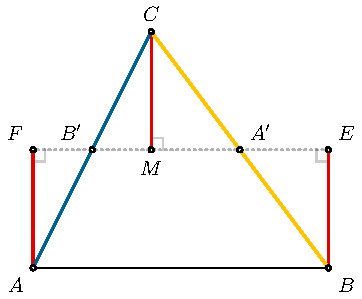
\includegraphics[scale=1]{figures/figure-triangle_to_rectangle.pdf}
\end{center}

\begin{theorem}
	任何長方形可以剪接成正方形。
\end{theorem}
\begin{proof}
	考慮以下圖形:
	\begin{center}
		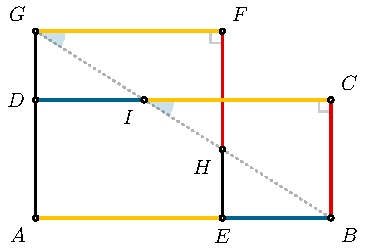
\includegraphics[scale=1]{figures/figure-rectangle_to_square.pdf}
	\end{center}
	我們想將 $\square{ABCD}$ 拼剪成正方形 $\square{AEFG}$。
	作法如下:
	\begin{enumerate}[label=(\arabic*)]
		\item 將 $\square{ABCD}$ 沿著 $\overline{BG}$ 切開。
		\item 將 $\triangle{BCI}$ 平移到 $\triangle{HFG}$。
		\item 將 $\triangle{BHE}$ 沿著 $\overline{HE}$ 剪下。
		\item 將 $\triangle{BHE}$ 平移到 $\triangle{IGD}$。
	\end{enumerate}
	這個操作之所以可以執行,建立在 $\triangle{BCI}\cong\triangle{HFG}$ 上。
	顯然地,這兩個三角形相似,所以我們只要證明他們其中一對對應的邊相等即可。
	首先注意到 $\triangle{DGI}\sim\triangle{CBI}$,所以
	\begin{align*}
		\overline{DG}:\overline{BC} = \overline{DI}:\overline{CI}
		\implies
		\overline{DG}\cdot\overline{CI} = \overline{BC}\cdot\overline{DI}。 \tag*{$\odot$}
	\end{align*}
	再注意到 $\square{ABCD}$ 與 $\square{AEFG}$ 的面積相等,故
	\begin{align*}
		( \overline{BC} + \overline{DG} )^2
		&= \overline{BC} \cdot ( \overline{CI} + \overline{DI} ) \tag*{(面積相等)}\\
		&= \overline{BC}\cdot\overline{CI} + \overline{BC}\cdot\overline{DI}  \\
		&= \overline{BC}\cdot\overline{CI} + \overline{DG}\cdot\overline{CI}  \tag*{(根據 $\odot$)}\\
		&= ( \overline{BC} + \overline{DG} )\cdot\overline{CI} \\
		\implies
		\overline{CI} &= \overline{BC} + \overline{DG} \tag*{($\overline{BC}+\overline{DG}\neq0$)} \\
		&= \overline{EF} = \overline{FG}。
	\end{align*}
	由於 $\overline{CI}=\overline{FG}$,可知 $\triangle{BCI}\cong\triangle{HFG}$。
\end{proof}

\begin{remark}
	考慮一個長寬比為 $5:1$ 的長方形,
	上述的作法還可行嗎?
	如果不可,遇到的問題是什麼,然後要怎麼修改作法呢?
\end{remark}

\begin{theorem}
	任兩個正方形可以剪貼成一個正方形。
\end{theorem}

\begin{center}
	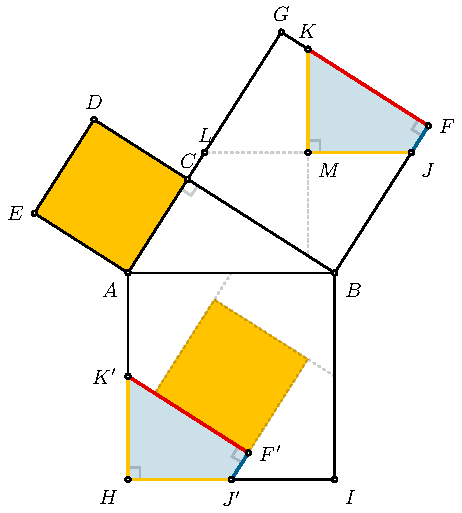
\includegraphics[scale=1]{figures/figure-pythagorean.pdf}
\end{center}

\begin{theorem}
	任何一個多邊形可以剪貼成任何一個多邊形。
\end{theorem}

\vfill\hfill\zhdate{2022/04/20}

\end{multicols*}
\end{document}
